\section{Понятие пограничного слоя}
	Движение вязких сред практически всегда связано с явлениями переноса в пограничном слое, где локализуются сопротивления трения, тепло- и массоотдачи. Понятие пограничного слоя впервые использовано Людвигом Прандтлем в статье, представленной 12 августа 1904 г., на третьем Международном конгрессе математиков в Гейдельберге, Германия. Классическим примером пограничного слоя является пограничный слой, который образуется на плоской пластине при обтекании ее поверхности жидкостью и пограничный слой в круглых трубах. Более сложным для исследования и математического описания является пограничный слой на поверхностях с различной кривизной (обтекание цилиндра, сферы и др. тел). Такой пограничный слой характеризуется большим градиентом давления и точкой отрыва, за которой производная и скорость потока меняют знаки. Так же значительно сложны и труднодоступны пограничные слои на поверхности раздела двухфазных и многофазных сред.
	
	Пограничный слой -- область течения вязкой жидкости с малой по сравнению с продольными размерами поперечной толщиной, образующаяся у поверхности обтекаемого твёрдого тела или на границе раздела двух потоков жидкости с различными скоростями или температурами. Пограничный слой характеризуется резким изменением в поперечном направлении скорости (динамический пограничный слой) или температуры (температурный пограничный слой).
	
	Чем меньше вязкость среды, тем тоньше гидродинамический пограничный слой и большее значение в этом слое имеет градиент скорости. Вне пограничного слоя градиент скорости невелик. Следовательно, силы трения здесь малы, и ими обычно пренебрегают. Между внешним потоком и пограничным слоем резкой границы нет, поскольку средняя скорость жидкости по сечению потока изменяется монотонно, без скачков. Обычно толщину пограничного слоя определяют условно, исходя из того, что на его внешней границе скорость составляет 99 \% от скорости внешнего потока.
	
	Значение пограничного слоя очень велико, так как он определяет гидродинамическое сопротивление при движении среды относительно твердого тела, а также сопротивление переносу массы и тепла. Введение этого понятия существенно упростило уравнения моделирования течение жидкости путём разделения потока на две области. Для описания пограничного слоя используются уравнения Навье-Стокса:
	\begin{align}
		& \frac{\partial u}{\partial x} + \frac{\partial v}{\partial y} + \frac{\partial w}{\partial z} = 0 \nonumber\\
		& u\frac{\partial u}{\partial x} + v\frac{\partial u}{\partial y} + w\frac{\partial u}{\partial z} = -\frac{1}{\rho}\frac{\partial p}{\partial x} + \nu(\frac{\partial^2 u}{\partial x^2} + \frac{\partial^2 u}{\partial y^2} + \frac{\partial^2 u}{\partial z^2}) \nonumber\\
		& u\frac{\partial v}{\partial x} + v\frac{\partial v}{\partial y} + w\frac{\partial v}{\partial z} = -\frac{1}{\rho}\frac{\partial p}{\partial y} + \nu(\frac{\partial^2 v}{\partial x^2} + \frac{\partial^2 v}{\partial y^2} + \frac{\partial^2 v}{\partial z^2})\nonumber\\
		& u\frac{\partial w}{\partial x} + v\frac{\partial w}{\partial y} + w\frac{\partial w}{\partial z} = -\frac{1}{\rho}\frac{\partial p}{\partial z} + \nu(\frac{\partial^2 w}{\partial x^2} + \frac{\partial^2 w}{\partial y^2} + \frac{\partial^2 w}{\partial z^2})
	\end{align}
	Существуют три вида течения в пограничном слое:
	\begin{itemize}
		\item ламинарное -- движение жидкости упорядочено, слои не смешиваются, частицы вращаются в пределах одного и того же тонкого слоя;
		\item турбулентное -- движение неупорядочено, происходит перемешивание частиц в поперечном направлении и весь пограничный слой беспорядочно завихрен;
		\item смешанное -- переходное состояние от ламинарного к турбулентному режиму движения.
	\end{itemize}

\section{Турбулентное состояние пограничного слоя}
	Ламинарное течение устойчиво только при некоторых условиях, определяемых значением критического числа Рейнольдса $Re_{cr}$. Обычно переход от ламинарного к турбулентному режиму течения жидкости в трубах наблюдается при $Re_{cr} \approx 2300$. Однако этот переход зависит от устойчивости исходного ламинарного течения по отношению к внешним возмущениям. Если вход в трубу сделать плавным, то ламинарное движение в трубе может поддерживаться при больших числах Рейнольдса, например до 24 000. Существенно влияют на $Re_{cr}$ и такие факторы, как градиент давления, форма канала, шероховатость его стенок, вдув и отсос пограничного слоя. 
	
	Турбулентное движение в пограничном слое возникает из-за нестабильности потока, которая проявляется в виде вихрей различных размеров и интенсивности. Эти вихри перемешивают слои жидкости, что приводит к увеличению переноса массы и энергии вдоль поверхности твердого тела. Параметры турбулентного потока в пограничном слое характеризуются такими величинами, как скорость, давление, плотность и температура. Важными параметрами являются также коэффициент трения, переноса тепла и массы. Турбулентное течение с большим числом Рейнольдса называют развитой турбулентностью.
	
	Для описания турбулентности используются уравнения Навье-Стокса, которые описывают законы сохранения массы, импульса и энергии для жидкости. Однако аналитическое решение этих уравнений возможно только для очень простых течений. В общем случае для описания турбулентных потоков применяются численные методы, такие как метод прямого численного моделирования или моделирование крупных вихрей. Одной из фундаментальных проблем гидродинамики турбулентных течений является проблема турбулентного переноса. Она связана с необходимостью описать перемещение частиц жидкости и массы, энергии и импульса в условиях сложных турбулентных потоков
	
	Существует каскадный перенос энергии, т.е. её передача от более крупных вихрей к более мелким. Наиболее крупные вихри получают энергию от осредненного течения, передают её всё более мелким, а наиболее мелкие диссипируют в тепло. Скорость этого процесса в силу хаотичности природы турбулентности также колеблется вокруг некой величины, при этом ее мгновенное значение может становиться отрицательным. Иными словами, в некоторые моменты времени энергия может передаваться от более мелких вихрей к более крупным, но эта флуктуация компенсируется более интенсивной передачей энергии по каскаду в другие моменты времени.

\section{Структура пограничного слоя}
	В турбулентном пограничном слое обычно выделяется несколько областей: внешняя и внутрення. Они отличаются друг от друга разными масштабами вихревых структур\cite{Белов2001}. 
	\begin{figure}[H]
		\centering
		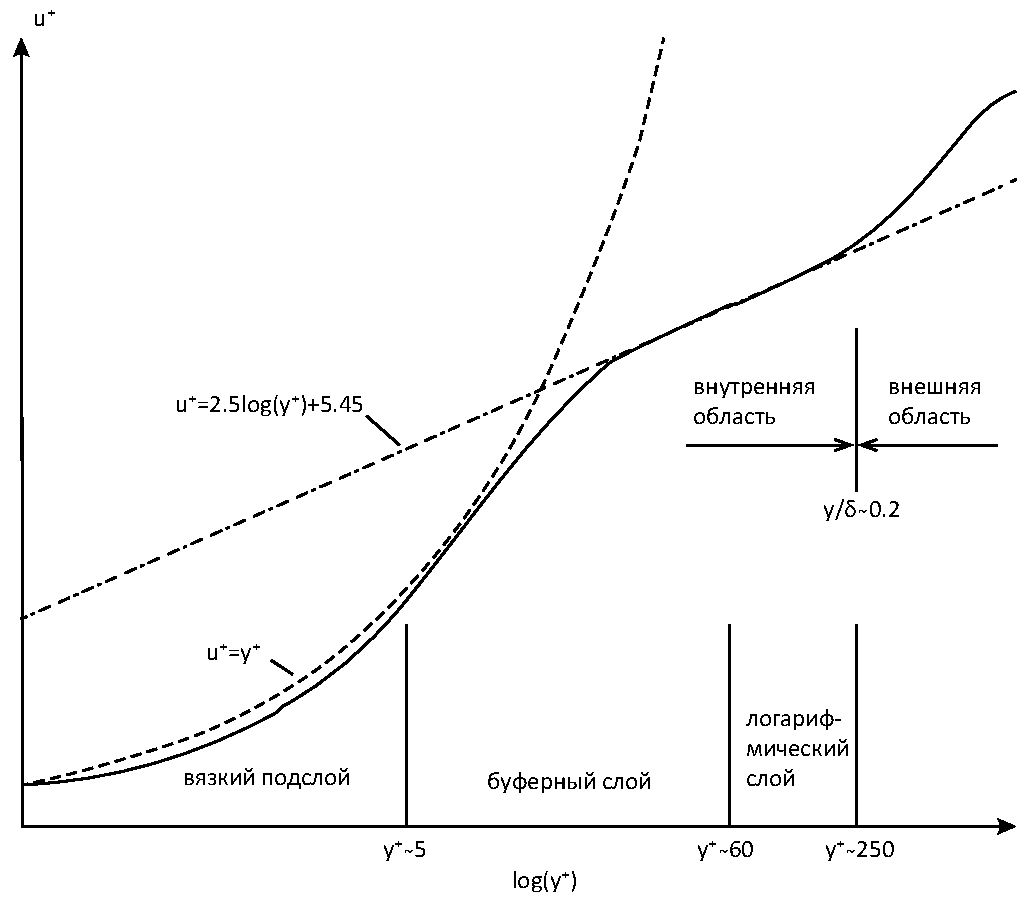
\includegraphics[width=0.7\linewidth]{../Assets/ПогранСлойRU}
		\caption{Схема слоя}
	\end{figure}
	Внутренняя область пограничного слоя занимает примерно 20\% от толщины всего слоя и в ней генерируется до 80\% энергии турбулентности. На формирование течения в пограничном слое основное влияние оказывают вязкость, теплопроводность и диффузионная способность жидкости. Внутри динамического пограничного слоя происходит плавное изменение скорости от её значения во внешнем потоке до нуля на стенке вследствие прилипания вязкой жидкости к твёрдой поверхности. Аналогично внутри пограничного слоя плавно изменяется температура.
			
\subsection{Внешняя область}

	Внешний слой является областью полностью развитого турбулентного течения, в котором распределение скорости описывается логарифмическим законом. Полное затухание возмущений во внешней области происходит на расстоянии, во много раз превышающем линейный масштаб турбулентности.
	
	Чтобы определить поток во внешней зоне, применяют фильтрованные или усредненные по Рейнольдсу уравнения Навье-Стокса. В то же время, профиль скорости во внутренней зоне сравнительно мало зависит от различных внешних условий, таких как числа Рейнольдса и градиент давления, что позволяет использовать универсальные соотношения (пристеночные функции) для связи параметров потока с расстоянием от стенки. Этот метод также базируется на гипотезе о локальном равновесии энергии турбулентных пульсаций и свойствах локальной изотропности диссипирующих вихрей.

\subsection{Внутрення область}

	Вязкий подслой, буферный и логарифмический слои составляют внутреннюю область пограничного слоя. Она характеризуется высокой скоростью переноса массы, импульса и тепла, что приводит к повышенной трению и потере энергии.
	\begin{align}
		v\frac{\partial u}{\partial y} \gg -\overline{u'v'} & \qquad\text{вязкий}\nonumber \\
		v\frac{\partial u}{\partial y} \approx -\overline{u'v'} & \qquad\text{буферный}\nonumber \\
		v\frac{\partial u}{\partial y} \ll -\overline{u'v'} & \qquad\text{логарифмический}
	\end{align}
	
	Существует два подхода к моделированию течения в пристеночной области. В первом подходе используются полуэмпирические формулы (пристеночные функции) для описания внутреннего слоя потока, в то время как во втором подходе модели турбулентности модифицируются таким образом, чтобы разрешать всю пристеночную область потока, включая вязкий подслой, при условии обеспечения необходимого разрешения сетки в пограничном слое. Такие модели турбулентности могут быть использованы для расчета турбулентных течений во всей расчетной области (включая пристеночную область течения).

\subsection{Свойства пограничного слоя}
	
	Толщина пограничного слоя трудно определима как в расчёте, так и в эксперименте. Для определения используются понятия: толщина вытеснения $\delta^*$ и толщина потери импульса $\theta$.
	\begin{equation}
		\delta^* = \int_{0}^{\infty}(1 - \frac{u}{U_0})dy \qquad \theta = \delta^{**} = \int_{0}^{\infty} \frac{u}{U_0}(1 - \frac{u}{U_0})dy
	\end{equation}
	Кроме того используется безразмерный параметр $H$:
	\begin{equation}
		H = \frac{\delta^*}{\theta}
	\end{equation}
	
	Число Рейнольдса характеризуется двумя величинами($Re_x$ и $Re_\theta$): расстоянием от начала $x$ и толщиной $\theta$.
	\begin{equation}
		Re_x = \frac{xU_0}{\nu} \qquad Re_\theta = \frac{\theta U_0}{\nu}
	\end{equation}
	
	Используя напряжение трения на стенке $\tau_w$ можем вычислить коэффициент трения $C_F$ и динамическую скорость $u_\tau$:
	\begin{equation}
		\tau_w = \nu\frac{\partial u}{\partial y}\bigg|_W \qquad C_F = \frac{\tau_w}{0.5\rho U_0^2} \qquad u_\tau = \sqrt{\frac{\tau_w}{\rho}}
	\end{equation}
	
	Не менее важной характеристикой пограничных слоев является продольный градиент давления:
	\begin{equation}
		\frac{dp}{dx} = -\rho U_0 \frac{dU_0}{dx}
	\end{equation}
	
	Часто на пограничные слои влияют такие факторы: кривизна поверхности $\kappa$, скорость закачки и откачки жидкости, шероховатость поверхности $k_s^+$(высота бугорков).
	\begin{equation}
		\kappa = \frac{\delta^*}{R} \qquad \frac{V_W}{u_\tau}, \frac{V_W}{U_0} \qquad k_s^+ = \frac{k_s u_\tau}{\nu}
	\end{equation}
	
	Важным свойством пограничного слоя является выполнение интегрального уравнения импульсов. Верно и обратное: если уравнение импульсов не выполняется, то уравнения плоского пограничного слоя также не верны для этого течения. Это может быть обусловлено разными причинами: трехмерность течения, его нестационарность, влияние вверх по потоку, изменение давления поперек пограничного слоя, влияние нормальных Рейнольдсовых напряжений и т.д.
	\begin{equation}
		\frac{d\theta}{dx} + \frac{dU_0}{dx}\cdot\frac{2 + H}{U_0}\theta - \frac{C_f}{2} = 0
	\end{equation}

\section{Локальное трение и перенос}
	% Про что писать найдено, нужна просто инфа, как можно больше и с формулами %
	
	Теоретическую основу описания процессов переноса в пограничном слое составляют фундаментальные законы сохранения и равновесия, одним из свойств которых является их инвариантность к масштабу и к взаимодействию с другими явлениями, т.е. структура математического описания пограничного слоя слабо зависит от контактного устройства.
	
	Для изучения влияния вихрегенераторов в турбулентном пограничном слое на локальное трение и перенос изучались следующие параметры: средняя скорость и её пульсация , напряжение трения на стенке $\tau_w$, коэффициент трения $C_F$ и динамическая скорость $u_\tau$.
	Для представления профилей компонент средней скорости и их пульсаций использовались безразмерные координаты $u^+$ и $y^+$:
	\begin{equation}
		u^+ = \frac{U}{u_\tau} \qquad y^+ = \frac{yu_\tau}{v}
	\end{equation}

\section{Методы моделирования}
	
	Несмотря на интенсивное развитие вычислительной техники и впечатляющие успехи, достигнутые в последние годы как в области построения эффективных численных алгоритмов, предназначенных для решения задач гидромеханики и тепломассопереноса, так и в разработке сопутствующего математического обеспечения (генераторы сеток, интерактивные системы ввода данных и систем визуализации результатов расчетов), проблема численного моделирования турбулентности, как и на протяжении многих предшествующих десятилетий, по-прежнему остается одной из наиболее сложных и актуальных проблем механики жидкостей. В отличие от ламинарных течений однофазной среды (жидкости), расчет которых, благодаря отмеченным выше достижениям, стал во многом рутинной процедурой, надежное предсказание характеристик сложных турбулентных течений, представляющих наибольший практический интерес все еще остается сложным.
	\begin{figure}[H]
		\centering
		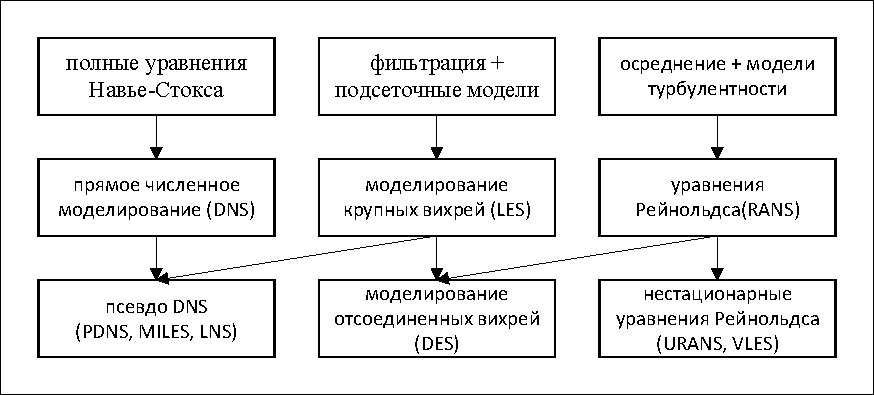
\includegraphics[width=0.9\linewidth]{../Assets/СхемаМетодов}
		\caption{Виды методов по уравнениям}
		\label{fig:cheme}
	\end{figure}
	
	Среди основных методов численного моделирования трехмерных турбулентных течений можно выделить: прямое численное моделирование (DNS), моделирование крупных вихрей (LES) и решение осредненных по Рейнольдсу уравнений Навье-Стокса (RANS). Имеются также различные промежуточные подходы, сочетающие в себе те или иные черты RANS, LES и DNS, например, метод моделирования отсоединенных вихрей (DES), и ряд других, не имеющих должного физического обоснования и потому не получивших широкого распространения.

\subsection{DNS}
	
	Прямое численное моделирование(DNS) предполагает решение полных нестационарных трехмерных уравнений Навье-Стокса, позволяющее получить мгновенные характеристики турбулентного потока. Проблемы с широким использованием DNS связаны с высокими требованиями к используемой разностной схеме, удовлетворением начальных и граничных условий, а также ограниченными ресурсами вычислительной техники. Расчетная область при этом должна быть достаточно протяженной, чтобы вместить наибольшие масштабы турбулентности, а шаг интегрирования по времени должен иметь порядок колмогоровского масштаба.
	
	\begin{table}[H]
		\begin{center}
			\begin{tabular}{|c|c|c|c|c|}
				\hline
				Re & 6.6$\times10^3$ & 2.0$\times10^4$ & 1.0$\times10^5$ & 1.0$\times10^6$\\
				\hline
				Кол-во узлов сетки & 2$\times10^6$ & 4$\times10^7$ & 3$\times10^8$ & 1.5$\times10^3$\\
				\hline
				150 MFlops & 37 ч & 740 ч & 6.5 лет & 3000 лет\\
				\hline
				1 TFlops & 20 с & 400 с & 8.3 ч & 4000 ч\\
				\hline
			\end{tabular}
		\end{center}
		\caption{Затраты времени при различных параметрах}
	\end{table}

\subsection{RANS}
	
	В инженерных приложениях широко используются математические модели, основанные на численном решении осредненных по Рейнольдсу уравнений Навье-Стокса(RANS). При использовании уравнений Рейнольдса основной интерес проявляется к динамике крупномасштабных вихрей, ответственных за переносные свойства турбулентных течений. При замыкании уравнений Рейнольдса рассматриваются масштабы длины, типичные для энергосодержащих вихрей, в которых $Re\gg1$ (за исключением пристеночных областей). Для учета пристеночного влияния диссипирующих вихрей и энергосодержащих вихрей при $Re\sim1$ используются демпфирующие функции.
	% Пересмотреть уравнения и/или найти другие более полезные %
	Уравнения Навье-Стокса:
	\begin{align}
		&\frac{\partial u_i}{\partial x_i} = 0 \nonumber\\
		&\rho\frac{\partial u_i}{\partial t} + \rho u_j \frac{\partial u_i}{\partial x_j} = - \frac{\partial p}{\partial x_i} + \frac{\partial}{\partial x_j}(\mu\frac{\partial u_i}{\partial x_j})
	\end{align}
	Для выполнения уравнений Навье-Стокса необходимо соблюдение двух условий:
	\begin{enumerate}
		\item Среда должна быть сплошной.
		\item Выполнение обобщённого реологического закона Ньютона.
	\end{enumerate}
	Применив к уравнениям осреднение Рейнольдса получим:
	\begin{align}
				&\frac{\partial u_i}{\partial x_i} = 0 \nonumber\\
				&\rho\frac{\partial u_i}{\partial t} + \rho u_j \frac{\partial u_i}{\partial x_j} = - \frac{\partial p}{\partial x_i} + \frac{\partial}{\partial x_j}(\mu\frac{\partial u_i}{\partial x_j} - \rho\overline{u_i' u_j'})
	\end{align}
	
	Для замыкания этой системы уравнений необходимо определить шесть различных компонент симметричного тензора турбулентных напряжений. Именно выражение этих компонент через параметры осредненного потока и называется моделью турбулентности. Ниже представлена таблица с основными этапами развития теории.
	
	\begin{table}[H]
		\begin{center}
			\begin{tabular}{|c|c|c|}
				\hline
				Год & Ученые & Что изучено\\
				\hline
				1877 & Буссинеск Ж. В. & гипотеза Буссинеска\\
				\hline
				1895 & Рейнольдс О. & осреднение по Рейнольдсу\\
				\hline
				1925 & Прандтль Л. & теория пути смешивания Прандтля\\
				\hline
				1930 & Карман Т. & формула Кармана\\
				\hline
				1942 & Колмогоров А. Н. & формула Колмогорова, модель $k$-$\omega$\\
				\hline
				1951 & Ротта & первая модель Рейнольдсовых напряжений\\
				\hline
				1956 & Клаузер & формула Клаузера\\
				\hline
				1956 & Ван-Дрист & демпфирующий множитель\\
				\hline
				1974 & Лондер Б. и Сполдинг Д. & модель $k$-$\epsilon$\\
				\hline
			\end{tabular}
		\end{center}
		\caption{Этапы развития теории}
	\end{table}
	
	Появление огромного количества моделей привело к необходимости выбора. Для этого необходимо провести сравнительный анализ моделей. Однако при попытке тестирования естественным образом возникают определенные трудности. Во-первых, необходимо выбрать течения, для которых известен набор достоверных экспериментальных данных, свободных от погрешностей, а также выбрать критерии для сравнения моделей. Во-вторых, необходимо провести серийные расчеты этих течений с использованием разных моделей турбулентности и при этом быть уверенными в независимости результата от программной реализации задачи. Результатом такой работы должны явиться рекомендации по области применимости тех или иных моделей турбулентности.

\subsection{LES}
	
	Метод моделирования крупных вихрей(LES) был предложен Иосифом Смагоринским в 1963 году. Он основан на двух предположениях. Первый предполагает, что течение можно разделить на движение крупных и мелких вихрей. Крупные вихри, находящиеся под прямым воздействием граничных условий и несущие в себе максимум рейнольдсовых напряжений, рассчитываются. Мелкомасштабная турбулентность считается изотропной и имеющей универсальные характеристики, а потому менее критичной и более поддающейся моделированию. Другой  заключается в возможности аппроксимации нелинейных взаимодействий между крупными и мелкими вихрями только по крупным вихрям с использованием подсеточных моделей(SGS). Иначе говоря, принимается гипотеза о статистической независимости крупных и мелких вихрей.
	
	Статистика крупных вихрей обычно не чувствительна к подсеточному моделированию за исключением пристеночной области. Имеющиеся подсеточные модели корректно предсказывают не только осредненные характеристики потока (первые и вторые моменты), но также и флуктуации интегральных характеристик, например, коэффициентов сопротивления и подъемной силы\cite{Fureby2000}.
	
	Мелкомасштабное движение исключается из уравнений Навье-Стокса при помощи применения операции фильтрации и моделируются с помощью подсеточных моделей. На рисунке \ref{fig:lesfilter} показан принцип работы фильтров, где $g(x)$ - исходный вариант, $f(x)$ - после фильтрации.\\
	\begin{figure}[H]
		\centering
		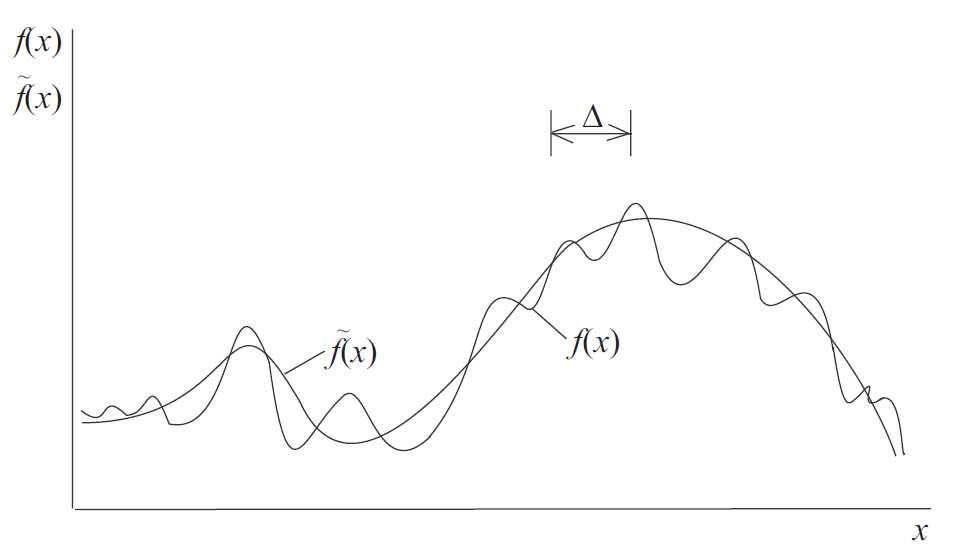
\includegraphics[width=0.7\linewidth]{../Assets/ФильтрацияLES}
		\caption{Исключение мелкомасштабных движений фильтрацией}
		\label{fig:lesfilter}
	\end{figure}
	
	Уравнение фильтра, применимое к пространственно временному полю $\phi(x,t)$ представлено ниже:
	\begin{equation}
		\overline{\phi(x,t)} = \int_{-\infty}^{\infty}\int_{-\infty}^{\infty}\phi(r,t')G(x - r, t - t')dt'dr
	\end{equation}
	В данном случае $G$ - ядро, характерное для каждого типа фильтра.
	
	Решение, полученное с помощью LES, содержит более богатую информацию по сравнению с решением на основе уравнений Рейнольдса, например, не только характеристики среднего течения (поля скорости, концентрации, температуры, давления) и распределения рейнольдсовых напряжений, но также и спектральные характеристики (спектры пульсаций скорости и давления), двухточечные моменты, временные и пространственные масштабы турбулентности.

\subsection{DES}
	
	Характерные для отрывных течений крупномасштабные нестационарные трехмерные вихревые структуры определяются конкретными граничными условиями и геометрическими характеристиками рассматриваемых течений и не могут быть описаны в рамках таких моделей. Это стимулируют поиск и разработку гибридных подходов, сочетающих в себе экономичность RANS и универсальность LES.
	
	В методе моделирования отсоединенных вихрей (DES) в области присоединенного пограничного слоя метод функционирует в режиме уравнений Рейнольдса, а в области отрыва потока переходит в LES. При этом достигается сочетание лучших качеств обоих подходов -- высокая точность и экономичность уравнений Рейнольдса в области присоединенного пограничного слоя и универсальность LES в отрывной области. Хотя DES, в отличие от RANS, является принципиально нестационарным трехмерным подходом, необходимые для его реализации сетки в пристеночной области совпадают с сетками, необходимыми для решения уравнений Рейнольдса, и являются на много порядков меньшими, чем сетки, требуемые для разрешения мелких пристенных вихрей в рамках LES. По мере измельчения сетки DES асимптотически приближается к LES и далее к DNS. Конкретные реализации DES основаны на использовании модели турбулентной вязкости Спаларта-Аллмараса и модели Ментера\cite{Strelets2001}.
	
	Как следует из названия метода DES, он создавался для расчета отрывных течений. Именно такие течения лучше других подходят для этого метода. Во-первых, наличие массированного отрыва в большинстве случаев приводит к его пульсациям, как следствие этого, к возникновению автоколебательного течения с крупными когерентными структурами. Во-вторых, наличие отрывной зоны позволяет обойти проблему создания турбулентных пульсаций на входе в LES области.

\subsection{Оценка производительности}
	
	Оценка количества узлов сетки и временных шагов, необходимых для реализации DNS и LES, показывает сложность проблемы с вычислительной точки зрения.
	
	\begin{table}[H]
		\begin{center}
			\begin{tabular}{|c|c|c|c|c|}
				\hline
				Метод & Число узлов сетки & Число шагов по времени & Готовность\\
				\hline
				RANS & $10^7$ & $10^3$ & 1985\\
				\hline
				DES & $10^8$ & $10^4$ & 2000\\
				\hline
				LES & $10^{11.5}$ & $10^{6.7}$ & 2045\\
				\hline
				DNS & $10^{16}$ & $10^{7.7}$ & 2080\\
				\hline
			\end{tabular}
		\end{center}
		\caption{Перспектива применения методов}
	\end{table}
	Готовность означает практическое применение метода с затратой времени не более суток.
	Для оценки необходимых вычислительных ресурсов (например, быстродействия и объема оперативной памяти) возьмем расчетную сетку 100$\times$100$\times$100 узлов($10^6$ точек). В каждом узле необходимо вычислить около 10 функций (составляющие скорости, плотность, давление, температуру, характеристики турбулентности, концентрации компонентов смеси). Значения неизвестных функций находятся в результате решения системы нелинейных уравнений, что требует от 200 до 1000 арифметических операций. За один шаг по времени необходимо выполнить $10^{10}$ операций с плавающей точкой. Для исследования развития процесса во времени требуется до 1000 временных шагов. В результате, выполнение одного расчета требует $10^{13}$ операций с плавающей точкой. Для проведения одного расчетного варианта компьютер с производительностью 100 МФлопc($10^8$ операций с плавающей точкой в секунду) затратит $10^7$ секунд. Для проведения расчета за 100 минут потребуется компьютер с производительностью 0.1 ТФлопс.